\documentclass[10pt]{article}
\usepackage[utf8]{inputenc}
\usepackage{amsmath}
\usepackage{amsfonts}
\usepackage{amssymb}
\usepackage{graphicx}

\begin{document}
\section*{Software Development Overview}

\paragraph*{}This experiment card uses an ST Micro STM32L151ZDT6 Low-Power ARM Processor to perform all required tasks.  The STM32L1 allows for 32-bit processing and DMA peripherals with a 48Kb SRAM for processing the JPEG data.  Table \ref{spec_table} shows the basic specifications of the processor.

\paragraph*{}As described in the hardware description, the processor has several hardware peripherals attached to it other than the satellite IHU: 8Mb SPI MRAM, 3Mb dual-port DRAM FIFO, and the OV7670 camera sensor.  These interfaces and connections are described in Table \ref{bus_table}

\begin{table}
	\centering
	\caption{STM32L1 Specifications}
	\begin{tabular}{ll}
	\hline
	Property & Specification \\
	\hline
	\hline
	Speed & 32 MHz \\
	Rated Current & 238 uA/MHz \\
	Program Flash & 382KB ECC \\
	Memory & 48KB ECC SRAM \\
	EEPROM & 12KB ECC EEPROM \\
	Footprint & LQFP144\\
	\end{tabular}
	\label{spec_table}
\end{table}

\begin{table}
	\centering
	\caption{Peripheral Specifications}
	\begin{tabular}{llll}
	\hline
	Peripheral & Bus Type & $\mu$C Interface & Speed \\
	\hline
	\hline
	MRAM & SPI & DMA Hardware SPI & 32MHz \\
	FIFO & 8-bit Wide Clocked & Software Bit-Bang & 3.2MHz \\
	OV7670 & I2C-like Two-Wire & Software Bit-Bang & 25kHz \\
	IHU & UART & DMA Hardware UART & 38.4kbaud \\
	\end{tabular}
	\label{bus_table}	
\end{table}

\paragraph*{}A real-time operating system (RTOS) is used for task management and hardware abstraction.  The software team chose ChibiOS (http://www.chibios.org/), a GPLv3 RTOS, for use on this stem.  The HAL and other device management features of the operating system were intuitive to learn.  However, in prototyping and development there were some adaptation problems with the ChibiOS version used.  After migrating from STM32L1-DISCOVERY boards to actual design prototypes it was discovered that ChibiOS did not fully implement the High-Density STM32L1 devices.  The OS source had to be modified to expand the PAL and HAL to accommodate the expanded device capabilities.

\paragraph*{}Programming and development of this system was done entirely on linux-based systems.  An ARM cross-compiling toolchain was built for GCC; our specific toolchain is available at http://wq3c.net/arm-cc.tar.bz2 .  To flash the STM32L1-DISCOVERY and the design prototypes, the ST-Link (v2) interface was used.  Similar to our discovery with ChibiOS, our selected flash utility ( https://www.github.com/texane/stlink ) did not fully support the high density devices.  The stlink project was forked and modified with necessary modifications for programming our device ( https://www.github.com/mitchd/stlink ).

\begin{table}
	\centering
	\caption{ChibiOS Key Features}
	\begin{tabular}{l}
		\hline
		\hline
		1.2-5.5 KiB Kernel Size \\
		Preemptive scheduling, round-robin for like priorities \\
		128 priority levels \\
		Mutexes, semaphores, events, message queues \\
		Thread-safe heap \\
		Hardware abstraction layer with STM32L1 support \\
		GPLv3 \\
	\end{tabular}
\end{table}
	
\section*{System Architecture}

\subsection*{Threads and Tasks}
\begin{figure}
	\centering
	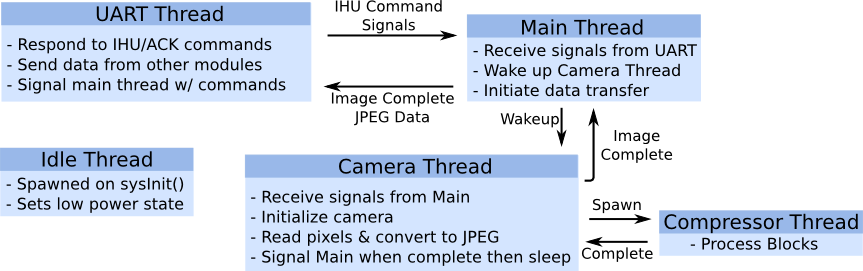
\includegraphics[width=0.8\textwidth]{task_diagram.png}
	\caption{Task Diagram}
	\label{task_diagram}
\end{figure}
\paragraph*{}Figure \ref{task_diagram} describes the task diagram for the imaging experiment.  Multiple threads are utilized to take advantage of different priority levels provided by the RTOS and increase code modularity.  A flowchart in Figure \ref{flowchart} describes in greater detail the sequence of events for capturing and transmitting a picture.  Not shown on the flowchart is a default command to take a picture.  Due to systems operations and simplification, it is assumed that when the experiment is powered on, a picture is requested.

\begin{figure}
	\centering
	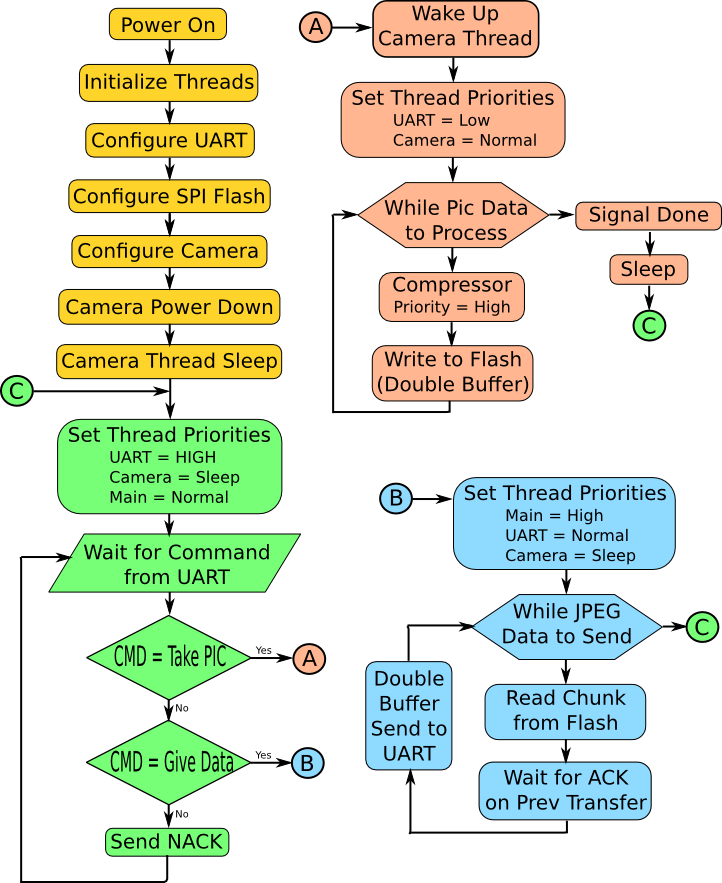
\includegraphics[width=0.9\textwidth]{flow_chart.png}
	\caption{System Operation Flowchart}
	\label{flowchart}
\end{figure}

\subsection*{Image Processing}

\paragraph*{}The OV7670 camera module provides 4:2:2 YUV data to the processor through the DRAM FIFO.  Due to limitations in the FIFO storage space, the image is divided into two parts for processing.  JPEG compression is achieved by reading eight horizontal lines from the FIFO and passing to the JPEG compressor.  For the purpose of this description, these eight-line segments are called `scan lines.'  The JPEG algorithm processes images in eight by eight pixel chunks: performing a discrete cosine transform, quantizing the results, then huffman coding the quantized data.  This particular implementation uses a library `jpegant' ( https://code.google.com/p/jpegant/ ) which implements an integer approximation of the DCT.  It should be noted that the Google Code version of jpegant is GPLv2 (which is incompatible with GPLv3), the author was contacted and we were authorized a GPLv3 release of his code.
\paragraph*{}The JPEG compression routine makes use of a little-used feature in the JPEG specification: the RSI marker.  RSI is the `restart interval' of the huffman coding.  This allows for missing data in the received image, while the image will not look complete it will not render the entire image useless.  The target compression ratio for the 640x480 image is at least 15:1 compression; each scan line should be less than 1023 bytes.

\subsection*{Data Storage}

\paragraph*{}Image data is stored on the 8MB MRAM module after processing.  A predefined address in the MRAM module contains a data structure which contains important information about the image: a memory map of each scan line (beginning and end addresses) and a checksum.  Should time warrant before final release, ECC will be implemented in the MRAM storage and retrieval routines.
\end{document}